\section{Ball Swinging in a Horizontal Circle}
\label{act8.3.1}
\note{For Activity~\ref{act8.3.1} (\about\unit[70]{min})
}{
\subsection*{Learning Goals:}
\begin{itemize}
\item Gain understanding of circular motion using conical pendulum
\end{itemize}
}
\begin{overview}

	\textbf{Overview:} Remember the Mass Swinging in a Horizontal Circle in \hyperref[MassCircle]{Activity \ref{MassCircle}} on page \pageref{MassCircle}? We already started analyzing the forces acting on the ball in that activity. As a sort-of culmination of the semester, we return to this scenario to continue our analysis of the forces on the ball using several of the models we've learned to use.
	
\end{overview}

\noindent\textbf{Phenomenon:} Ball on a string, swinging in a horizontal circle at constant speed. The experiment shows that as the ball moves faster, $\theta$ becomes larger, and the tension in the string increases.

%\begin{wrapfigure}[6]{r}{6cm}
%        \centering
%        \vspace{-\baselineskip}
\begin{center}
			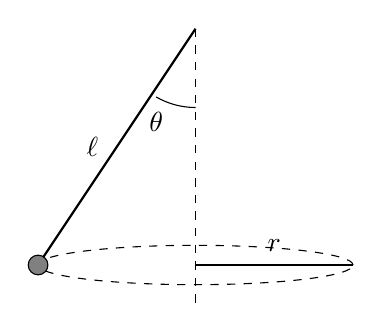
\begin{tikzpicture}{r}{1}
				% Reference Measurements
				\draw[dashed] (2,3.5) -- (2,0);
				\draw[dashed] (2,0.5) ellipse (2cm and 0.25cm);
				\draw[thin] (2,0.5) -- (4,0.5) node[midway,above=1.5pt] {$r$};
				\draw[thin] (2,2.5) arc (270:240:1) node[below=2pt] {$\theta$};
				
				% Ball & String
				\draw[thick] (2,3.5) -- (0,0.5) node[midway,left=3pt] {$\ell$};
				\draw[fill=gray] (0,0.5) circle (0.125cm);
			\end{tikzpicture}
\end{center}
%	  \end{wrapfigure}


\subsection*{What model/approach would you use?}

Suppose you are interested in how the tension in the string depends on the angle $\theta$ that the string makes with the vertical direction. Which approach do you think would help you make progress with this question: energy conservation, momentum %or angular momentum
conservation, or Newton's 2nd law?\\
	\note{}{You need to know about forces in detail.  Not necessarily the time dependence, but just the forces themselves.  The motion in the horizontal direction is changing directions.  The motion in the vertical direction is not changing at all.  Either the impulse equals change in momentum approach or Newton�s 2nd law approach would work here.  Both involve looking in detail at the forces}

\noindent Discuss in your group what information you specifically need, and which models/approaches can give you that information. Start by thinking about the specific motion and what is required to produce this motion. (Note that rotational velocity -- how fast the ball swings around the circle -- is assumed constant. What does this imply?)

\subsection*{Use the model}
	\note{For~\ref{act8.3.1-2a}}{Something like 
\begin{center}
\includegraphics[width=.1\textwidth]{U8/figs/ballonstring.png}
\end{center}	
	}
Carry out the analysis using whichever approach/model you have decided on.
\begin{enumerate}
	\item Put a properly labeled \forcediag{} for the ball on the board.
	\label{act8.3.1-2a}

	
	\item \label{act8.3.1-2b} Use the \forcediag{} to develop \textbf{two} mathematical relationships (one for the vertical direction and one for the horizontal direction). You will need to figure out (or remember) the direction of the acceleration of an object traveling in a circle at constant speed. The magnitude of this acceleration is $a_\text{centripetal} = \frac{v_\text{tangential}{}^2}{r}$.\\(Notice $v_\text{tangential}$ refers to the \emph{tangential} speed of the ball).
\note{For \ref{act8.3.1-2b}}{Using either momentum conservation or Newton�s 2nd, student should find the relation for the horizontal direction will be $F_{by string} \sin \theta = mv^2/r$ and for the vertical direction will be $F_{by string}\cos\theta - F_{by earth} = 0$.}
	
	\item \label{act8.3.1-2c}Does the force of the string on the ball equal the force of the Earth on the ball? If not, what does?
	\note{For \ref{act8.3.1-2c}}{
	No $F{by string} = mg/\cos\theta$
	}
	
\WCD
\vspace{2pt}

	\item \label{8.3.1-2d}Illustrate using vectors what happens to the tension in the string ($\vec{F}_\text{string on ball}$) when the tangential speed of the ball increases. Think about how the two relationships in \eqref{act8.3.1-2a} can both be satisfied.
	\note{For \ref{8.3.1-2d}}{Illustrate using vectors what happens when the tangential speed of the ball increases.  Think about how the two relationships in \ref{act8.3.1-2b} can both be satisfied.
\begin{center}
\includegraphics[width=.6\textwidth]{U8/figs/twovectors.png}
\end{center}	
}
	
	\item \label{8.2.1-2e}Develop a short explanation of why the angle of the string (from the vertical direction) changes when the tangential velocity is increased significantly. Check this out with the real ball and string.
	\note{For \ref{8.3.1-2e}}{
	The main point is that the vertical component of the strings force must always balance the weight.  In the horizontal direction, the force must increase as the tangential velocity increases.  The only way both of these conditions can be satisfied is if the angle the string makes with the vertical increases towards 90� as the 
	}
\end{enumerate}

\WCD
